%----------------------------------------------------------------------------------------
%	PACKAGES AND THEMES
%----------------------------------------------------------------------------------------
\documentclass[aspectratio=169,xcolor=dvipsnames]{beamer}

\usepackage{hyperref}
\usepackage{graphicx} % Allows including images
\usepackage{booktabs} % Allows the use of \toprule, \midrule and \bottomrule in tables
\usepackage{bm}% bold math
\usepackage{physics}
\setlength{}{}%
\usepackage{siunitx}
\usepackage[inline]{asymptote}
\usepackage{multirow}
\usepackage{tikz}
\usepackage{pgfplots, pgfplotstable}
\usepackage{hyperref}
\usepackage{natbib}
% \usepackage{amsthm}
\usepackage{amssymb}
\usepackage{amsmath}
\usepackage{cancel}

\usepackage{xcolor} % more colors

\definecolor{my-blue}{RGB}{93,169,233}
\definecolor{my-pink}{RGB}{238,118,116}
\definecolor{my-green}{RGB}{0,191,0}
\definecolor{my-orange}{HTML}{FE5F55}
\definecolor{background}{HTML}{f2f2f2}
\definecolor{my-yellow}{HTML}{F6BD60}
\definecolor{dark-blue}{HTML}{00008B}
\definecolor{my-maroon}{HTML}{800000}

\usepackage[breakable,many]{tcolorbox}
% Math

\tcbset{simple/.style={
            breakable,
            enhanced,
            outer arc=0pt,
            arc = 0pt,
            colback=background, % Background color
            colframe=background, % Border Color
            coltitle=black, % Title Color
            fonttitle=\bfseries,
            attach title to upper,
            after title={:\ },
            segmentation style={dashed, gray},
        }
}

\tcbset{color-labeled/.style={
            breakable,
            enhanced,
            outer arc=0pt,
            arc=0pt,
            colframe=#1,
            colback=#1!5,
            attach title to upper,
            coltitle=#1!200,
            after title={\medbreak},
        }
}

\tcbset{one-sided-color/.style={
            breakable,
            enhanced,
            boxrule=0pt,
            frame hidden,
            borderline west={2pt}{0pt}{#1},
            colback=#1!10,
            coltitle=#1!200,
            after title={:\ },
            sharp corners,
            attach title to upper,
        }
}

%%%%%%%%%%%%%%%%%%%%%%%%%%%%%%%%%%%%%%%%%%%%%%%%%%%%%%%%%%
%%%%%%%%%%%%%%%%%%   Box Definitions %%%%%%%%%%%%%%%%%%%%%
%%%%%%%%%%%%%%%%%%%%%%%%%%%%%%%%%%%%%%%%%%%%%%%%%%%%%%%%%%

\newtcolorbox[auto counter]{examplee}{
    simple,
    title=\textbf{Example} \thetcbcounter,
    % add a `\thetcbcounter` to the end if you want to keep track of numberings.
}

\newtcolorbox{mathematica}{
    simple,
    title=\textbf{Mathematica Snippet},
    % add a `\thetcbcounter` to the end if you want to keep track of numberings.
}

\newtcolorbox[auto counter]{experiment}{
    simple,
    title=\textbf{Experiment:},
    % add a `\thetcbcounter` to the end if you want to keep track of numberings.
}

\newtcolorbox[auto counter]{custom-big}[1][]{
    color-labeled=my-yellow,
    title=\textbf{{#1}},
}

\newtcolorbox{definitionn}{
    one-sided-color=my-green,
    title=\textbf{Definition},
}

\newtcolorbox{mnemonic}{
    one-sided-color=my-green,
    title=\textbf{Mnemonic},
}

\newtcolorbox{theoremm}{
    one-sided-color=my-blue,
    title=\textbf{Theorem},
}


\newtcolorbox[auto counter]{proposition}{
    one-sided-color=my-blue,
    title=\textbf{Proposition} \thetcbcounter,
}

\newtcolorbox[auto counter]{corollaryy}{
    one-sided-color=my-blue,
    title=\textbf{Corollary} \thetcbcounter,
}

\newtcolorbox[auto counter]{lemmaa}{
    one-sided-color=my-blue,
    title=\textbf{Lemma} \thetcbcounter,
}

% \newtcolorbox{proposition}{
%     one-sided-color=my-green,
%     title=\textbf{Proposition},
% }

%----------------------------------------------------------------------------------------
%	TITLE PAGE
%----------------------------------------------------------------------------------------

% The title
\title[short title]{Wormholes in General Relativity: Just how feasible are they?}
% \subtitle{Subtitle}

\author{QiLin Xue}
\institute[UofT] % Your institution may be shorthand to save space
{
    % Your institution for the title page
    University of Toronto
    \vskip 3pt
}
\date{\today} % Date, can be changed to a custom date


%----------------------------------------------------------------------------------------
%	PRESENTATION SLIDES
%----------------------------------------------------------------------------------------

\begin{document}

\begin{frame}
    % Print the title page as the first slide
    \titlepage
\end{frame}
%------------------------------------------------
\section{First Section}
%------------------------------------------------

\begin{frame}{Motivation}
    \begin{itemize}
        \item Consider an inter-universe wormhole: allows for maximal symmetry
    \end{itemize}
    \begin{center}
        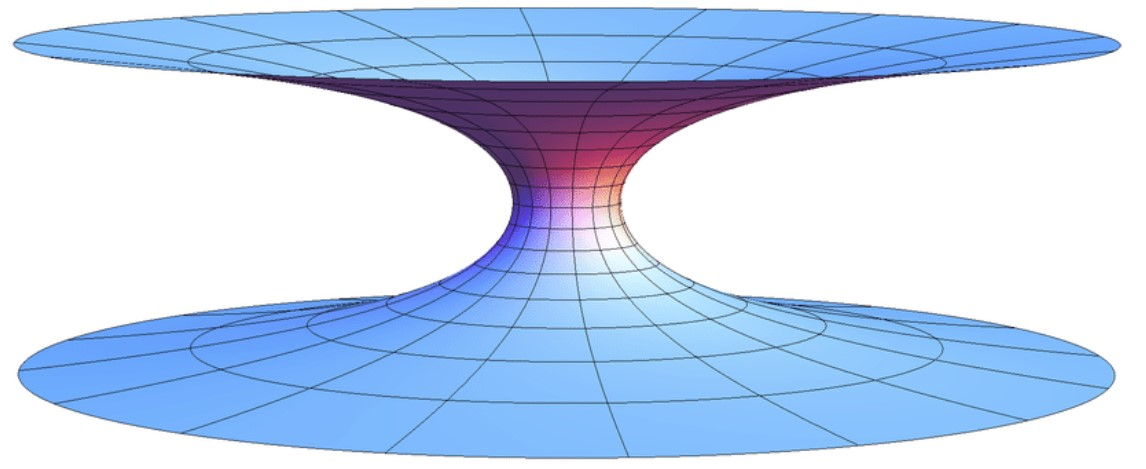
\includegraphics[width=0.6\linewidth]{figures/embedding.jpg}
    \end{center}
    \begin{itemize}
        \item Metric given by 
        \begin{equation}
            \dd{s}^2 = -e^{2\Phi(r)}\dd{t}^2 + \frac{\dd{r}^2}{1-b(r)/r} + r^2\left(\dd{\theta}^2 + \sin^2\theta\dd{\varphi}^2\right),
        \end{equation} 
    \end{itemize}
\end{frame}

\begin{frame}{Metric}
    \begin{equation*}
        \dd{s}^2 = -e^{2\Phi(r)}\dd{t}^2 + \frac{\dd{r}^2}{1-b(r)/r} + r^2\left(\dd{\theta}^2 + \sin^2\theta\dd{\varphi}^2\right),
    \end{equation*}
    \begin{itemize}
        \item Connects the two universes at $r=r_0$
        \item Universes can be identified by having two coordinate charts $[r_0,\infty)$ 
        \item Proper radial distance given by
        \begin{equation}
            \ell(r) = \pm \int_{r_0}^{r} \frac{\dd{r}}{\sqrt{1-b(r)/r}}
        \end{equation}
        \item Define radius of throat to be $r(\ell = 0)=r_0$
    \end{itemize} 
\end{frame}

\begin{frame}{Metric}
    \begin{equation*}
        \dd{s}^2 = -e^{2\Phi(r)}\dd{t}^2 + \frac{\dd{r}^2}{1-b(r)/r} + r^2\left(\dd{\theta}^2 + \sin^2\theta\dd{\varphi}^2\right),
    \end{equation*}
    \begin{proposition}
        In some open neighbhourhood near the throat $(r_0,r_*),$ the following inequality holds:
        \begin{equation}
            b'(r) < \frac{b(r)}{r}
        \end{equation}
    \end{proposition}
\end{frame}

\begin{frame}{Curvature}
    \begin{itemize}
        \item Stress energy tensor is $T=\text{diag}(\rho,p_r,p,p).$ Einstein's equation gives at the throat,
        \begin{align}
            8\pi \rho &= \frac{b'(r_0)}{r_0^2} \label{eq:Gtt}\\ 
            8\pi p_r &= -\frac{1}{r_0^2} \\ 
            8\pi p &= \frac{1}{2r_0^2}(1+r_0\Phi'(r_0))(1+b'(r_0)).
        \end{align}
        \item Eqaution \ref{eq:Gtt} gives 
        \begin{equation}
            b(r) = b(r_0) + 2\int_{r_0}^{r}4\pi \rho r^2\dd{r} \equiv 2m(r)
        \end{equation}
    \end{itemize}
\end{frame}

\begin{frame}{Energy Conditions}
    \begin{proposition}
        At the throat of the wormhole, the following inequality holds:
        \begin{equation}
            \rho + p \le 0.
        \end{equation}
    \end{proposition}
    \begin{itemize}
        \item Violates the null energy and weak energy condition,
        \begin{equation}
            \rho + p_i \ge 0.
        \end{equation}
        \item Turns out \textit{all} energy conditions are broken. The average null energy condition gives over any null curve $\Gamma,$ 
        \begin{equation}
            I_{\Gamma} = \int_{\Gamma} (\rho-\tau)\xi^2 \dd{\lambda} = -\frac{1}{4\pi}\int_{r_0}^{\infty}\frac{1}{r^2}e^{-\Phi(r)}\sqrt{1-\frac{b(r)}{r}}\dd{r}\ge 0.
        \end{equation}
        \item Only examples of energy conditions being broken are in QFT. Thus, modern wormholes are typically a \textit{quantum gravity} problem.
    \end{itemize}
\end{frame}
%------------------------------------------------

\begin{frame}{Traversability}
    Requirements:
    \begin{itemize}
        \item Traversable in a short amount of time.
        \item Weak tidal forces.
    \end{itemize}
    Tidal forces are the main problem, and we get the conditions:
    \begin{align*}
        |\Phi'| &\le \frac{2gr_0}{(1-b'(r))L} \\
        v^2 &\le \frac{2gr_0^2}{(1-b'(r))L}
    \end{align*}
\end{frame}

\begin{frame}{Constant Redshift Solution}
    Consider the case where $\Phi(r) = \Phi_0.$
    \begin{itemize}
        \item Numerous possible shape functions, i.e.
        \begin{equation}
            b(r) = \sqrt{b_0r}
        \end{equation}
        \item This gives 
        \begin{equation}
            \rho + p_r = -2p
        \end{equation}
        which is satisfied globally.
    \end{itemize}
\end{frame}

\begin{frame}{(Almost) Schwarzschild}
    Consider the metric 
    \begin{equation}
        \dd{s}^2 = -\left(1-\frac{r_0}{r} + \frac{\epsilon}{r^2}\right)\dd{t}^2 + \frac{\dd{r}^2}{1-\frac{r_0}{r}} + r^2\left[\dd{\theta}^2 + \sin^2\theta \dd{\varphi}^2\right]
    \end{equation}
    We can bound 
    \begin{equation}
        I_{\Gamma} > -\frac{1}{4\pi r_0}
    \end{equation}
\end{frame}
\begin{frame}{[Extra] Neglected History}
    \begin{itemize}
        \item Universe is a 3-sphere embedded in $\mathbb{R}^4.$ Spatial part of metric is (taking a $\theta=\frac{\pi}{2}$ slice)
        \begin{equation}
            \dd{\sigma}^2 = R_0^2\left(\dd{\psi}^2 + \sin^2\psi\dd{\varphi}^2\right)
        \end{equation}
        \item This surface is generated by a curve. Let $z$ point in direction of axis of rotation, and $R$ point in the direction perpendicular to $z$, in the same plane as circle.
        \begin{equation}
            \frac{dz}{dr} = \tan\psi
        \end{equation}
        \item For a Schwarzschild metric, spatial part is 
        \begin{equation}
            \dd{\sigma}^2 = \frac{\dd{r}^2}{1-2M/r} + r^2\dd{\varphi}^2.
        \end{equation}
        \item Consider the substitution 
        \begin{equation}
            \cos^2\psi = 1 - \frac{2M}{r}
        \end{equation}
    \end{itemize}
\end{frame}
\begin{frame}{[Extra] Neglected History}
    \begin{itemize}
        \item Universe is a 3-sphere embedded in $\mathbb{R}^4.$ Spatial part of metric is (taking a $\theta=\frac{\pi}{2}$ slice)
        \begin{equation}
            \dd{\sigma}^2 = R_0^2\left(\dd{\psi}^2 + \sin^2\psi\dd{\varphi}^2\right)
        \end{equation}
        \item This surface is generated by a curve. Let $z$ point in direction of axis of rotation, and $R$ point in the direction perpendicular to $z$, in the same plane as circle.
        \begin{equation}
            \frac{dz}{dr} = \tan\psi
        \end{equation}
        \item For a Schwarzschild metric, spatial part is 
        \begin{equation}
            \dd{\sigma}^2 = \frac{\dd{r}^2}{1-2M/r} + r^2\dd{\varphi}^2.
        \end{equation}
        \item Consider the substitution 
        \begin{equation}
            \cos^2\psi = 1 - \frac{2M}{r}
        \end{equation}
    \end{itemize}
\end{frame}
\begin{frame}{[Extra] Neglected History}
    Solving the differential equation 
\begin{equation}
    \frac{d\psi}{dr} = \sqrt{\frac{2M}{r-2M}}
\end{equation} 
gives
\begin{equation}
    z^2 = 8M(r-2M),
\end{equation}
which is plotted in the figure below, for the case $M=1.$
\begin{center}
    \scalebox{0.6}{
    \begin{tikzpicture}[scale=1]
    \begin{axis}[
    legend pos=outer north east,
    axis lines = middle,
    xlabel = $r$,
    ylabel = $z$,
    variable = t,
    trig format plots = rad,
    xmin = 0,
    ]
    \addplot [
        domain=2:10,
        samples=100,
        color=blue,
        ]
        {sqrt(8*x-16)};
        \addplot [
            domain=2:10,
            samples=100,
            color=blue,
            ]
            {-sqrt(8*x-16)};
        \end{axis}
    \end{tikzpicture}
}
\end{center}
\end{frame}
\begin{frame}{[Extra] Neglected History}
    \begin{itemize}
        \item Universe is a 3-sphere embedded in $\mathbb{R}^4.$ Spatial part of metric is (taking a $\theta=\frac{\pi}{2}$ slice)
        \begin{equation}
            \dd{\sigma}^2 = R_0^2\left(\dd{\psi}^2 + \sin^2\psi\dd{\varphi}^2\right)
        \end{equation}
        \item This surface is generated by a curve. Let $z$ point in direction of axis of rotation, and $R$ point in the direction perpendicular to $z$, in the same plane as circle.
        \begin{equation}
            \frac{dz}{dr} = \tan\psi
        \end{equation}
        \item For a Schwarzschild metric, spatial part is 
        \begin{equation}
            \dd{\sigma}^2 = \frac{\dd{r}^2}{1-2M/r} + r^2\dd{\varphi}^2.
        \end{equation}
        \item Consider the substitution 
        \begin{equation}
            \cos^2\psi = 1 - \frac{2M}{r}
        \end{equation}
    \end{itemize}
\end{frame}
\begin{frame}{References}
    \nocite{*}
    \bibliographystyle{unsrt}%Used BibTeX style is unsrt
    \bibliography{sample}
\end{frame}
\end{document}